\documentclass[12pt]{article}
\usepackage[english]{babel}
\usepackage[utf8x]{inputenc}
\usepackage{amsmath}
\usepackage{graphicx}
\usepackage[a4paper]{geometry}

\usepackage{listings}
\usepackage{color}

\definecolor{dkgreen}{rgb}{0,0.6,0}
\definecolor{gray}{rgb}{0.5,0.5,0.5}
\definecolor{mauve}{rgb}{0.58,0,0.82}

\lstset{frame=tb,
  language=Matlab,
  aboveskip=3mm,
  belowskip=3mm,
  showstringspaces=false,
  columns=flexible,
  basicstyle={\small\ttfamily},
  numbers=none,
  numberstyle=\tiny\color{gray},
  keywordstyle=\color{blue},
  commentstyle=\color{dkgreen},
  stringstyle=\color{mauve},
  breaklines=true,
  breakatwhitespace=true,
  tabsize=3
}

\begin{document}
\begin{titlepage}

% definition of custom command for horizontal lines
\newcommand{\HRule}{\rule{\linewidth}{0.5mm}}

\center
% HEADING
\textsc{\LARGE University of Dublin,\\Trinity College}\\[1.0cm]

\includegraphics[width=0.2\textwidth]{logo.png}

\HRule \\[0.4cm]
\textsc{\Large JS Engineering: 3C1 Signals \& Systems}\\[0.25cm]
\textsc{\large S1: LTI Systems}\\[0.1cm]
\HRule \\[0.4cm]
 
% AUTHORS
\begin{minipage}{0.5\textwidth}
\begin{flushleft} \large
\emph{Author:}
\\Edmond \textsc{O'Flynn} 12304742
\end{flushleft}
\end{minipage}
~
\begin{minipage}{0.4\textwidth}
\begin{flushleft} 
\large
\emph{Lecturer:} \\
William \textsc{Dowling} 
\end{flushleft}
\end{minipage}\\[6cm]

% DATE
{\large \today}\\[2cm] 

% LOGO
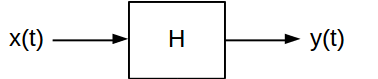
\includegraphics[width=0.5\textwidth]{lti.png}
\clearpage
\end{titlepage}

\newgeometry{top=1cm,left=1cm,bottom=2cm,right=1cm}
\tableofcontents
\addcontentsline{toc}{section}{References}
\thispagestyle{empty}
\cleardoublepage
\setcounter{page}{1}

\newgeometry{top=2cm,left=2cm,bottom=2cm,right=2cm}

\section{Abstract}

\section{Matlab}
In this laboratory, the scripting language \emph{Matlab} was used which gets compiled at its runtime. This makes for a language that is great for rapid-prototyping and extensive functionality within arithmetic, graphing, and graphical user interfaces. During this report, Matlab code snippets will be occasionally shown.

\section{Signals}
\subsection{Deterministic Sine Wave Signals}
\subsubsection{Plotting the Sine Wave $x_1$}
\begin{itemize}
\item Generate a deterministic signal $x_1=3sin(5t)$ over the range $0 \leq t \leq 6$ seconds.
\end{itemize}

\begin{lstlisting}
t = (0:0.01:6); % range 0-6 with steps of 0.01s
x1 = 3 * sin(5 * t);
figure(1); plot(t,x1);
title('Sine Wave Seconds v Voltages');
xlabel('Seconds (s)'); ylabel('Volts (V)');
\end{lstlisting}

\subsubsection{Properties}
\begin{itemize}
\item Voltage extrema
\begin{itemize}
\item Maximum: 3V
\item Minimum: -3V
\end{itemize}
\item Frequency
\begin{itemize}
\item 1.256s for 1 oscillation
\item $\frac{1}{1.256} \approx 0.796$Hz
\item Also determined from $\frac{5}{2\pi}$, where 5 refers to the factor before t, which also results in $0.796$ Hz
\end{itemize}
\item Periodicity
\begin{itemize}
\item Time for one cycle of the wave is 1.256s.
\end{itemize}
\end{itemize}

\subsubsection{Expanding to $x_2$}
\begin{itemize}
\item Generate a deterministic signal $x_2=Asin(\omega_{1}t + \phi)$ over the range $0 \leq t \leq 6$ seconds.
\end{itemize}

\begin{lstlisting}
w1 = 5;
phi = -3;
A = 3;
x2 = A * sin(w1 * t + phi);
hold on;plot(t,x2,'r');title('Sine Wave Seconds v Voltages');
xlabel('Seconds (s)');ylabel('Volts (V)');
\end{lstlisting}

Note that the same plot is overlaid using the hold on command for the plot given a previous one.

\subsubsection{Properties}
\begin{itemize}
\item Frequency
\begin{itemize}
\item 1.256s for 1 oscillation
\item $\frac{1}{1.256} \approx 0.796$Hz
\item Also determined from $\frac{5}{2\pi}$, where 5 refers to the factor before t, which also results in $0.796$ Hz
\end{itemize}
\item Periodicity
\begin{itemize}
\item Time for one cycle of the wave is 1.256s.
\end{itemize}
\item Differences between $x_1$ and $x_2$
\begin{itemize}
\item $x_1$ is a regular sine wave that has no offsets or lags. $x_2$ however, is offset such that it has almost become inverted. They two signals share the same amplitude and frequency.
\end{itemize}
\item Is there a phase lag?
\begin{itemize}
\item Yes there is. $x_2$ contains a lag $\phi$ that is not present in $x_1$.
\end{itemize}
\item Is this a delay or an advance?
\begin{itemize}
\item This is a delay with respect to $x_1$.
\end{itemize}
\end{itemize}

\subsubsection{Delay}
Between $x_2$ and $x_1$, there is about 0.657s lag time. I picked one point common to both signals (-3V), and recorded the difference in time between the two signals to reach this. 

\subsubsection{Expanding Further to $x_3$}
\begin{itemize}
\item Generate a deterministic signal $x_3=Asin(\omega_{1}t + \phi)$ over the range $0 \leq t \leq 6$ seconds.
\end{itemize}

\begin{lstlisting}
w1 = 5;
phi = -3 + (2 * 3.14);
A = 3;
x3 = A * sin(w1 * t + phi);
hold on;plot(t,x3,'r');title('Sine Wave Seconds v Voltages');
xlabel('Seconds (s)');ylabel('Volts (V)');
\end{lstlisting}

\subsubsection{Properties}
The function generated by $x_3$ is identical to $x_2$. The only difference is that $x_3$ has been shifted by $2\pi$.
\section{Linear Time Invariant Systems}
\subsection{LTI Systems}

\subsection{Discussion}

\subsection{Results}

\subsection{Gain \& Phase as a Function of a Frequency}

\section{Discussion}
\begin{enumerate}
\item What does frequency and phase mean with respect to a pure sinusoidal signal?
\item How does an LTI system affect a pure sinosoid?
\item What is the definition of an LTI system?
\item What do the terms \emph{phase shift} and \emph{gain} mean?
\item How are the step and impulse response of system characterised?
\end{enumerate}

\section{Bibliography}
\begin{thebibliography}{3}
\bibitem{streetmanb}
  Ben G. Streetman \& Sanjay Kumar Banerjee,
  \emph{Solid State Electronic Devices, 6th edition},
  Prentice Hall (2006),
  Pages 154-388.
\end{thebibliography}
\end{document}
